\section{HP Causality}

\begin{thm}
Given an event structure $\es$, a cause $X = S \vdash\,e$
where $(S, e) \in \vdash$, and an effect $Y = S_f$
where $S_f \in \conf{\es}$, $X$ is a cause of $Y$
(according to the HP definition) if there is at least one path
from $m_{S,e}$ to $x_{S_f}$ in the causal graph of $\es$.
\end{thm}

\begin{proof}
We check the conditions of HP causality for the given cause and effect.

\begin{itemize}
  \item \textbf{AC1:} Both the cause and effect hold in the factual scenario;
  therefore, this condition is satisfied.
\end{itemize}

For AC2.\{a,b\}, assume $(W, w, x')$ is the witness discussed by HP.

\begin{itemize}  
  \item \textbf{AC2.a:} The idea here is to restrict the causal graph
  such that the effect holds as long as the cause.
  
  Assume the path from cause to effect is as follows:
  \[
    m_{S,e} \rightarrow
    r_{S_1,S_2} \rightarrow
    x_{S_2} \rightarrow
    r_{S_2, S_3} \rightarrow
    \cdots \rightarrow
    r_{S_{k-1}, S_k} \rightarrow x_{S_k} = x_{S_f}
  \]

  We also define $W$ as:
  \[ \left( \In{r_{S_1, S_2}} \setminus \set{x_{S_1}, m_{S,e}} \right) \cup
    \left( \bigcup_{i=2}^k \In{x_{S_i}} \setminus \set{r_{S_{i-1}, S_i}} \right) \]
   
  The elements of $W$ are shown with dotted boxes in Fig. \ref{fig:witness}.
  All variables in $W$ are set to False ($w$ is an all-False valuation).
  $x'$ sets $r_{S,e}$ to False as well.
  
  \begin{figure}
\centering
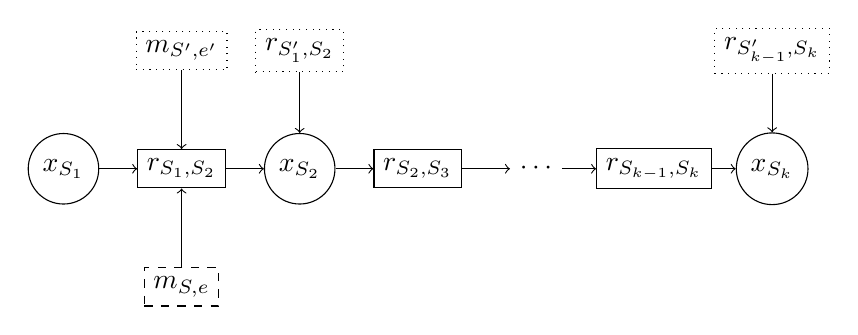
\begin{tikzpicture}
  \tikzset{
    _x/.style={circle,draw},
    r/.style={rectangle,draw},
    m/.style={rectangle,draw,dashed},
    w/.style={rectangle,draw,dotted},
  };
  \node[_x] (x-S1)       at (-1.5,0)  {$x_{S_1}$};
  \node[_x] (x-S2)       at (1.5,0)   {$x_{S_2}$};
  \node[_x] (x-Sk)       at (7.5,0)   {$x_{S_k}$};
  \node[m]  (m-S-e)      at (0,-1.5)  {$m_{S,e}$};
  \node[r]  (r-S1-S2)    at (0,0)     {$r_{S_1,S_2}$};
  \node[r]  (r-S2-S3)    at (3,0)     {$r_{S_2,S_3}$}; 
  \node[r]  (r-Sk-1-Sk)  at (6,0)     {$r_{S_{k-1},S_k}$};
  \node[w]  (m-S'-e')    at (0,1.5)   {$m_{S',e'}$};
  \node[w]  (r-S'1-S2)   at (1.5,1.5) {$r_{S'_1,S_2}$};
  \node[w]  (r-S'k-1-Sk) at (7.5,1.5) {$r_{S'_{k-1},S_k}$};
  \node     (dots)       at (4.5,0)   {$\cdots$};

  \draw[->] (x-S1)       -- (r-S1-S2);
  \draw[->] (m-S-e)      -- (r-S1-S2);
  \draw[->] (m-S'-e')    -- (r-S1-S2);
  \draw[->] (r-S1-S2)    -- (x-S2);
  \draw[->] (r-S'1-S2)   -- (x-S2);
  \draw[->] (x-S2)       -- (r-S2-S3);
  \draw[->] (r-S2-S3)    -- (dots);
  \draw[->] (dots)       -- (r-Sk-1-Sk);
  \draw[->] (r-Sk-1-Sk)  -- (x-Sk);
  \draw[->] (r-S'k-1-Sk) -- (x-Sk);
\end{tikzpicture}
\caption{Elements of $W$}
\label{fig:witness}
\end{figure}
    

  With the witness described above, we can see that the effect $x_{S_f}$
  is also valuated as False; therefore, condition AC2.a is satisfied.
  
  
  \item \textbf{AC2.b:} After setting $m_{S,e}$ to True,
  while maintaining $w$ as all-False, $x_{S_f}$ is valuated to True again.
  The \textit{validating} edges for $x_{S_f}$ are shown with thick lines
  in Fig. \ref{fig:ac2.b}. Observe that, re-setting any variable $v \not\in W$
  does \textbf{not} \textit{invalidate} the specified path for $X_{S_f}$.

  \input{./fig/fig:ac2.b}

  \item \textbf{AC3:} As our cause is a singleton,
  this condition is also satisfied.
\end{itemize}

\end{proof}